\documentclass[border=4pt]{standalone}

% --- packages (mirror these in gpu.meta.json "requires") ---
\usepackage{tikz}

% --- palette (canonical source: reference/color-palettes/color-palettes.md; light variant) ---
\definecolor{otblue}{HTML}{0072B2}
\definecolor{otorange}{HTML}{E69F00}
\definecolor{otteal}{HTML}{009E73}
\definecolor{otpurple}{HTML}{CC79A7}
\definecolor{otgray}{HTML}{5A5A5A}

\begin{document}
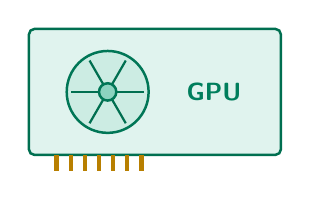
\begin{tikzpicture}[line width=0.9pt]
  % board
  \filldraw[draw=otteal!70!black, fill=otteal!12, rounded corners=2pt] (0,0) rectangle (3.2,1.6);
  % fan: hub, blades, rim
  \begin{scope}[shift={(1.0,0.8)}]
    \filldraw[draw=otteal!75!black, fill=otteal!20] (0,0) circle[radius=0.52];
    \foreach \a in {0,60,...,300}{\draw[otteal!70!black, line width=0.8pt] (0,0) -- (\a:0.46);}
    \filldraw[draw=otteal!75!black, fill=otteal!45] (0,0) circle[radius=0.11];
  \end{scope}
  % label
  \node[font=\sffamily\small\bfseries, text=otteal!80!black] at (2.35,0.8) {GPU};
  % gold edge connector (bottom)
  \foreach \i in {0,...,6}{\draw[otorange!80!black, line width=1.5pt] (0.35+\i*0.18,0) -- +(0,-0.2);}
\end{tikzpicture}
\end{document}
